\documentclass[12pt]{article}

% Configuración básica
\usepackage[spanish]{babel}
\usepackage[utf8]{inputenc}
\usepackage[T1]{fontenc}
\usepackage{geometry}
\usepackage{setspace}
\usepackage{hyperref}
\usepackage{enumitem}
\usepackage{graphicx}
\usepackage[section]{placeins} 
\usepackage{float}

\geometry{letterpaper, margin=2.5cm}
\onehalfspacing

% Datos del informe (puedes modificarlos)
\title{Avance 8 \\ Documentación técnica de procesos y desarrollos}
\author{David Armando Ramírez Navarrete}
\date{16 de febrero de 2026}

\begin{document}

\maketitle

\section*{Resumen}
El presente informe técnico documenta la elaboración y revisión de documentación técnica asociada a procesos de validación, pruebas y control de cambios, desarrollada durante el periodo de prácticas profesionales. La actividad se centró en la organización, estructuración y mantenimiento de información técnica mediante el uso de herramientas colaborativas de hoja de cálculo, con el propósito de asegurar la trazabilidad, consistencia y claridad de los procesos documentados.

El trabajo evidencia competencias en redacción técnica, organización de la información y comunicación profesional, así como la aplicación de buenas prácticas de documentación en un entorno técnico-profesional. Asimismo, se resalta la importancia de la documentación como soporte para el seguimiento de actividades, la verificación de resultados y la mejora continua de los procesos, sin comprometer información sensible ni sistemas propietarios.


\section*{Introducción}

La documentación técnica constituye un elemento fundamental dentro de los procesos de desarrollo, validación y mantenimiento de soluciones informáticas, ya que permite registrar de manera clara y estructurada las actividades realizadas, los criterios aplicados y los resultados obtenidos. Una documentación adecuada facilita la comprensión de los procesos, asegura la trazabilidad de la información y contribuye a la comunicación efectiva entre los distintos actores involucrados en un entorno técnico-profesional.

En el marco de las prácticas profesionales, se participó en la elaboración, revisión y actualización de documentación técnica relacionada con procesos de validación, pruebas y control de cambios. Dichas actividades se llevaron a cabo mediante el uso de herramientas colaborativas de tipo hoja de cálculo, las cuales permiten centralizar la información, mantenerla actualizada y respaldar cada etapa del proceso mediante evidencias documentales.

La presente evidencia tiene como propósito mostrar la capacidad para documentar procesos y desarrollos técnicos de forma organizada, clara y consistente, aplicando criterios de redacción técnica y buenas prácticas de documentación. El contenido presentado refleja la importancia de la documentación como soporte para el seguimiento de actividades, la verificación de resultados y la mejora continua de los procesos, sin comprometer información sensible ni sistemas propietarios.


\section*{Objetivo de la documentación}

El objetivo de la presente documentación es describir de manera clara, estructurada y técnica los procesos y actividades relacionadas con la validación, pruebas y control de cambios, desarrolladas durante las prácticas profesionales. A través de esta documentación se busca registrar de forma ordenada la información técnica, los criterios aplicados y las evidencias generadas en cada etapa del proceso.

Asimismo, la documentación tiene como finalidad servir como un medio de apoyo para el seguimiento, la verificación y la trazabilidad de las actividades realizadas, facilitando la comprensión del proceso por parte de los distintos participantes involucrados. De esta manera, se promueve la estandarización de la información, la correcta comunicación técnica y la reutilización del conocimiento documentado.

Finalmente, el documento pretende evidenciar la aplicación de buenas prácticas de documentación técnica, fortaleciendo competencias en redacción técnica, organización de la información y comunicación profesional, sin hacer referencia a sistemas propietarios ni a información sensible de la organización.


\section*{Alcance}

El alcance de la presente documentación se limita a la descripción general de los procesos y actividades relacionadas con la elaboración, revisión y control de documentación técnica utilizada durante las prácticas profesionales. El documento aborda aspectos funcionales y operativos de dichos procesos, incluyendo la organización de la información, la definición de criterios de validación y el registro de evidencias asociadas.

La documentación presentada no incluye nombres de sistemas, plataformas, herramientas propietarias ni información sensible, manteniendo un nivel de abstracción adecuado para fines académicos. Asimismo, no se describen implementaciones técnicas específicas ni configuraciones internas, sino que se enfoca en la metodología de documentación y en las buenas prácticas aplicadas.

El alcance del documento comprende únicamente las actividades desarrolladas durante el periodo de prácticas profesionales, sin considerar procesos externos o posteriores. De esta manera, la documentación busca servir como referencia académica que evidencie la capacidad para documentar procesos técnicos de forma estructurada, clara y profesional.


\section*{Descripción del proceso documentado}

El proceso documentado corresponde a la elaboración, revisión y control de documentación técnica asociada a actividades de validación, pruebas y seguimiento de cambios dentro de un entorno profesional. Dicho proceso tiene como finalidad asegurar que la información técnica generada durante las distintas etapas sea registrada de forma clara, estructurada y verificable, permitiendo su consulta y análisis posterior.

El proceso inicia con la definición de la estructura documental, en la cual se establecen los apartados necesarios para registrar información técnica relevante, tales como criterios de validación, tipos de prueba, responsables, fechas estimadas y evidencias asociadas. Esta estructura se implementa mediante hojas de cálculo colaborativas, las cuales funcionan como repositorios centralizados de información.

Posteriormente, se lleva a cabo el registro de la información técnica correspondiente a cada actividad, incluyendo la descripción de procesos, la planificación de pruebas, la identificación de componentes involucrados y la documentación de resultados esperados. Durante esta etapa se aplican criterios de consistencia y orden, con el objetivo de mantener la información homogénea y facilitar su interpretación.

Como parte del proceso, se realiza la revisión periódica de la documentación generada, verificando que los datos registrados sean coherentes, estén completos y cuenten con el soporte documental correspondiente. Esta revisión permite detectar inconsistencias, omisiones o desviaciones respecto a los criterios definidos, favoreciendo la corrección oportuna de la información.

Finalmente, el proceso contempla la integración de evidencias gráficas y registros de validación que respaldan las actividades documentadas. Estas evidencias permiten asegurar la trazabilidad entre los procesos ejecutados y la documentación generada, fortaleciendo el control del proceso y contribuyendo a una adecuada comunicación técnica entre los participantes involucrados.


\section*{Estructura de la documentación}

La documentación técnica elaborada durante las prácticas profesionales se organizó siguiendo una estructura clara y coherente, con el objetivo de facilitar su comprensión, mantenimiento y consulta. Dicha estructura permite identificar de manera ordenada los distintos elementos que conforman el proceso documentado, así como la relación entre actividades, criterios de validación y evidencias asociadas.

En una primera sección, la documentación contempla el registro general de la actividad o proceso, donde se describen aspectos como el objetivo, el tipo de actividad documentada y su contexto general. Esta información proporciona una visión inicial que permite comprender el propósito del documento y su aplicación dentro del proceso.

Posteriormente, se incluye una sección destinada a la planificación y control de actividades, en la cual se documentan los tipos de prueba, criterios de validación, responsables y fechas estimadas. Esta sección facilita el seguimiento del avance y permite identificar de manera oportuna el estado de cada actividad documentada.

La estructura también incorpora apartados específicos para el registro de resultados y observaciones, donde se documentan los hallazgos derivados de la ejecución de pruebas o revisiones técnicas. En estos apartados se detallan los resultados obtenidos, las incidencias detectadas y las acciones de seguimiento correspondientes, contribuyendo a la trazabilidad del proceso.

Finalmente, la documentación contempla un apartado para la integración de evidencias, en el cual se adjuntan o referencian elementos gráficos y registros que respaldan la información documentada. Esta organización estructurada permite asegurar la coherencia de la documentación, fortalecer el control del proceso y facilitar su reutilización como referencia técnica en actividades posteriores.


\section*{Resultados obtenidos}

Como resultado de la elaboración y revisión de la documentación técnica, se logró consolidar información relacionada con procesos de validación, pruebas y control de cambios en un formato estructurado, claro y accesible. La documentación generada permitió organizar de manera sistemática los criterios técnicos, las actividades realizadas y las evidencias asociadas a cada etapa del proceso.

Uno de los principales resultados fue la mejora en la trazabilidad de la información, al contar con registros que permiten relacionar actividades, responsables, fechas y resultados de forma coherente. Esta trazabilidad facilitó el seguimiento de las actividades documentadas y contribuyó a una mejor identificación del estado y avance de cada proceso.

Asimismo, la revisión continua de la documentación permitió detectar inconsistencias, información incompleta y oportunidades de mejora en el registro de datos técnicos. Estas observaciones fueron atendidas mediante ajustes y correcciones, fortaleciendo la calidad y confiabilidad de la documentación generada.

El uso de hojas de cálculo colaborativas como herramienta de documentación favoreció la centralización de la información y su actualización oportuna, reduciendo la dispersión de datos y mejorando la comunicación técnica entre los participantes del proceso. En conjunto, los resultados obtenidos evidencian la utilidad de la documentación técnica como soporte para el control, seguimiento y mejora continua de los procesos documentados.


\section*{Conclusiones}

La elaboración de documentación técnica desarrollada durante las prácticas profesionales permitió reforzar la importancia de registrar, organizar y mantener información técnica de manera clara y estructurada dentro de un entorno profesional. A través de este proceso, se evidenció que una documentación adecuada no solo facilita la comprensión de los procesos, sino que también contribuye al control, seguimiento y mejora continua de las actividades técnicas.

La participación en la creación y revisión de documentación relacionada con procesos de validación, pruebas y control de cambios favoreció el desarrollo de competencias en redacción técnica, organización de la información y comunicación profesional. Asimismo, el uso de herramientas colaborativas permitió centralizar la información, mantenerla actualizada y asegurar la trazabilidad entre actividades, criterios y evidencias documentadas.

Desde una perspectiva profesional, la documentación técnica se consolida como un elemento clave para la transferencia de conocimiento, la reducción de dependencias informales y la estandarización de procesos. En este sentido, la actividad realizada contribuyó al fortalecimiento del perfil profesional en el área de Ingeniería en Sistemas, al demostrar la capacidad para documentar procesos técnicos de forma responsable, estructurada y alineada a buenas prácticas, sin comprometer información sensible.


\section*{Referencias}

\begin{itemize}
    
    \item Agile Alliance. (n.d.). \textit{Agile Basics}.  
    Recuperado de: \url{https://agilealliance.org/agile101/agile-basics/}

    \item Atlassian. (n.d.). \textit{¿Qué es Scrum?}.  
    Recuperado de: \url{https://www.atlassian.com/es/agile/scrum}
    
    \item DataCamp. (n.d.). \textit{Python try-except: Exception handling explained}.  
    Recuperado de: \url{https://www.datacamp.com/tutorial/python-try-except}

    \item DataCamp. (n.d.). \textit{Python f-strings: Everything you need to know}.  
    Recuperado de: \url{https://www.datacamp.com/tutorial/python-f-string}

    \item DocuMind. (n.d.). \textit{Technical writing best practices}.  
    Recuperado de: \url{https://www.documind.chat/blog/technical-writing-best-practices}

    \item Google. (n.d.). \textit{Importar y exportar archivos}.  
    Recuperado de: \url{https://support.google.com/docs/answer/3093340?hl=es-419}

    \item Google. (n.d.). \textit{Convertir archivos a Google Docs}.  
    Recuperado de: \url{https://support.google.com/docs/answer/3093197?hl=es-419}

    \item Google Cloud. (n.d.). \textit{Cómo crear campos calculados en Looker Studio}.  
    Recuperado de: \url{https://docs.cloud.google.com/looker/docs/studio/tutorial-create-calculated-fields-in-looker-studio?hl=es-419}

    \item Google Cloud. (n.d.). \textit{Variables de resultado de consulta en Looker Studio}.  
    Recuperado de: \url{https://docs.cloud.google.com/looker/docs/studio/query-result-variables?hl=es-419}

    \item Google Cloud. (n.d.). \textit{Agregar, editar y solucionar problemas con campos calculados en Looker Studio}.  
    Recuperado de: \url{https://docs.cloud.google.com/looker/docs/studio/add-edit-and-troubleshoot-calculated-fields?hl=es-419}

    \item Google Workspace Developers. (n.d.). \textit{Google Apps Script overview}.  
    Recuperado de: \url{https://developers.google.com/apps-script/overview}

    \item Google Workspace Developers. (n.d.). \textit{Best practices for Google Apps Script}.  
    Recuperado de: \url{https://developers.google.com/apps-script/guides/support/best-practices}

    \item Google Workspace Developers. (n.d.). \textit{Custom menus in Google Sheets}.  
    Recuperado de: \url{https://developers.google.com/apps-script/guides/menus}

    \item Google Workspace Developers. (n.d.). \textit{Spreadsheet service}.  
    Recuperado de: \url{https://developers.google.com/apps-script/reference/spreadsheet}

    \item Google Workspace Developers. (n.d.). \textit{Calendar service}.  
    Recuperado de: \url{https://developers.google.com/apps-script/reference/calendar}

    \item Google Workspace Developers. (n.d.). \textit{Tasks API overview}.  
    Recuperado de: \url{https://developers.google.com/tasks}

    \item InvGate. (n.d.). \textit{Documentación técnica: mejores prácticas, formatos y ejemplos}.  
    Recuperado de: \url{https://blog.invgate.com/es/documentacion-tecnica}

    \item ISO. (n.d.). \textit{ISO 9001 — Documented information}.  
    Recuperado de: \url{https://www.iso.org/standard/62085.html}

    \item Python Software Foundation. (n.d.). \textit{Built-in exceptions}.  
    Recuperado de: \url{https://docs.python.org/3/library/exceptions.html}

    \item Python Software Foundation. (n.d.). \textit{PEP 8 -- Style Guide for Python Code}.  
    Recuperado de: \url{https://peps.python.org/pep-0008/}

    \item Real Python. (n.d.). \textit{Python Exceptions: An Introduction}.  
    Recuperado de: \url{https://realpython.com/python-exceptions/}

    \item Schwaber, K., \& Sutherland, J. (2020). \textit{La Guía Scrum}.  
    Recuperado de: \url{https://scrumguides.org/docs/scrumguide/v2020/2020-Scrum-Guide-Spanish-Latin-South-American.pdf}

    \item Scrum Guides. (n.d.). \textit{Scrum Guide – Downloads}.  
    Recuperado de: \url{https://scrumguides.org/download.html}

\end{itemize}


\appendix
\section{Evidencias gráficas de la Actividad 8}

\begin{figure}[H]
    \centering
    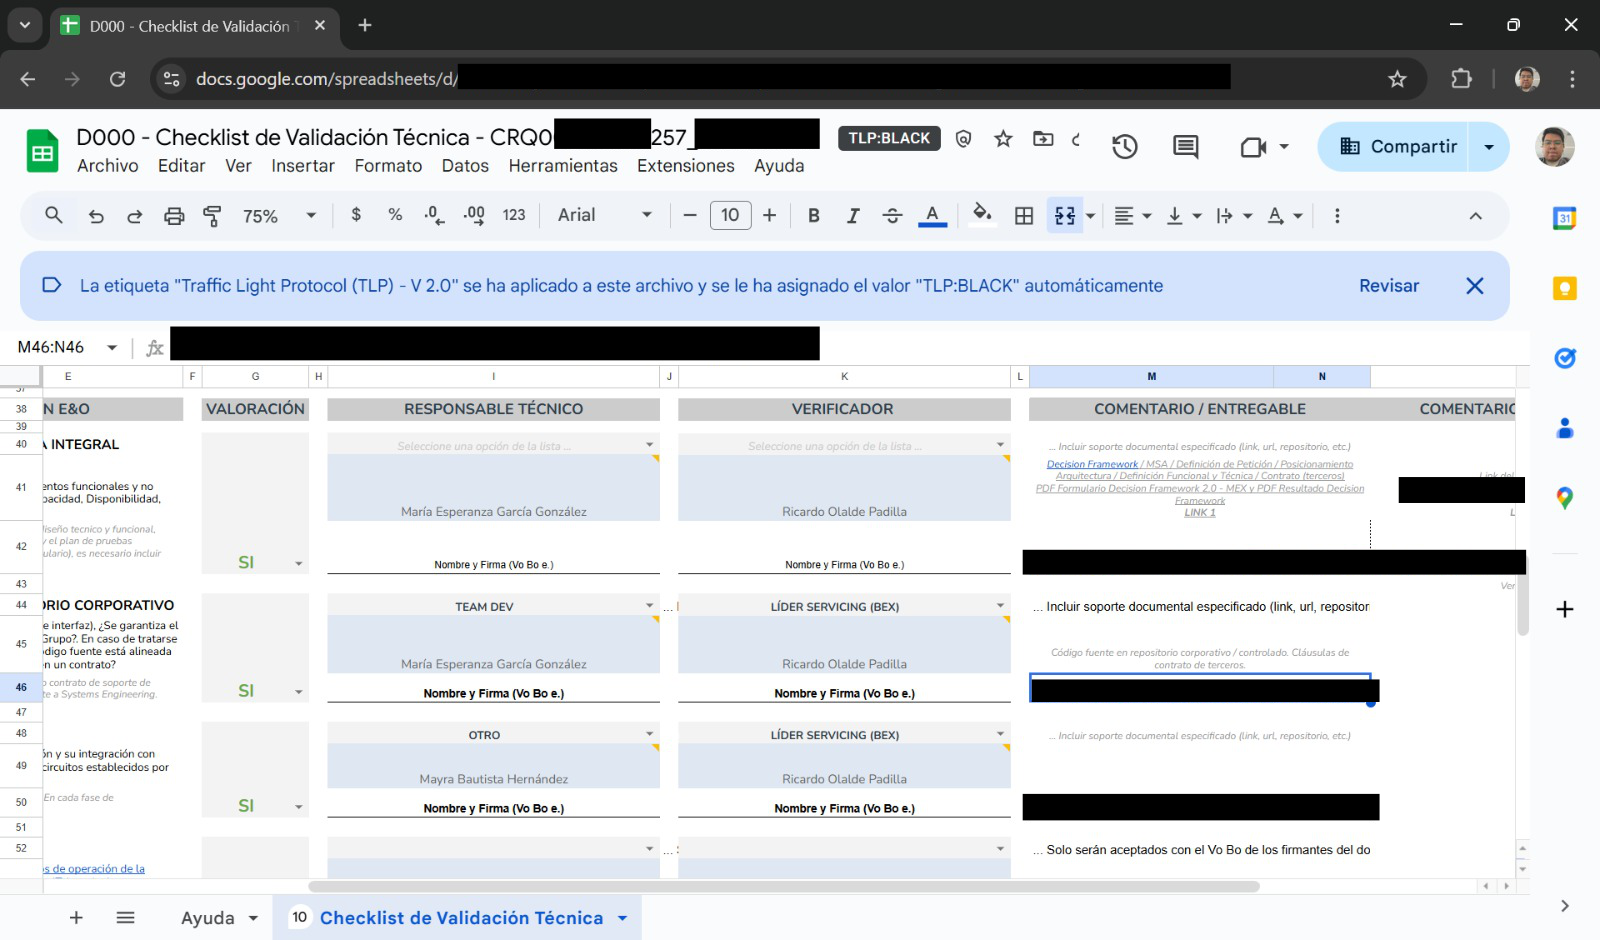
\includegraphics[width=0.95\textwidth]{E8/A8_1}
    \caption{Ejemplo de checklist de validación técnica documentado en hoja de cálculo colaborativa, utilizado para el control y seguimiento de criterios de revisión y aprobación técnica.}
\end{figure}

\begin{figure}[H]
    \centering
    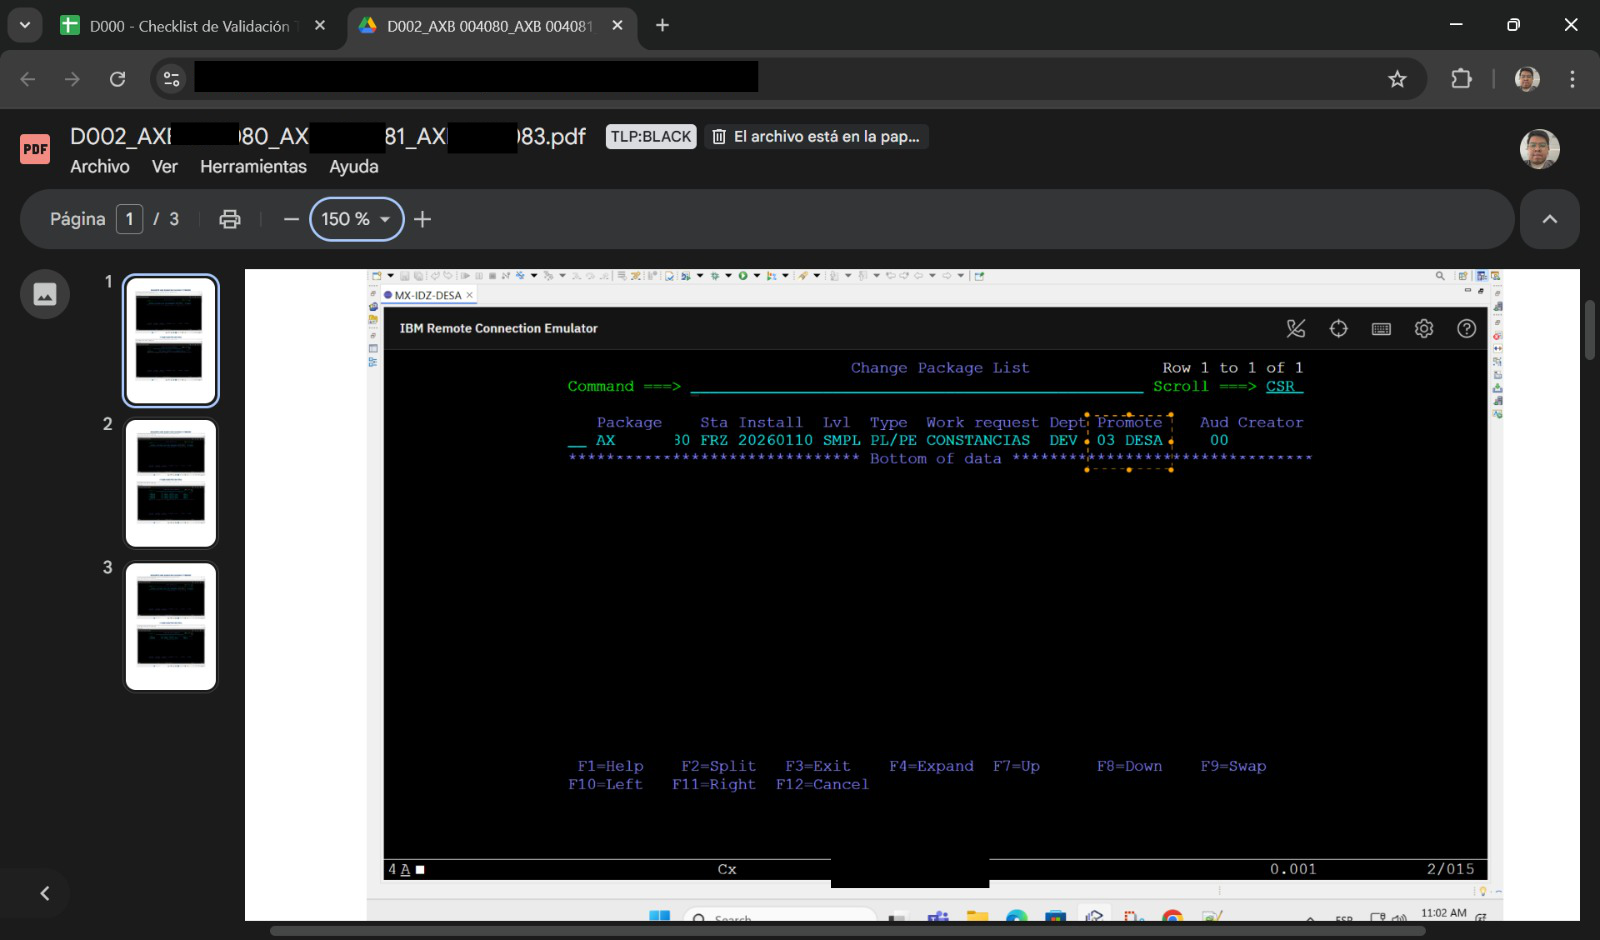
\includegraphics[width=0.95\textwidth]{E8/A8_2}
    \caption{Registro estructurado de validaciones técnicas y estatus de componentes, documentado como parte del proceso de control y trazabilidad de cambios.}
\end{figure}

\begin{figure}[H]
    \centering
    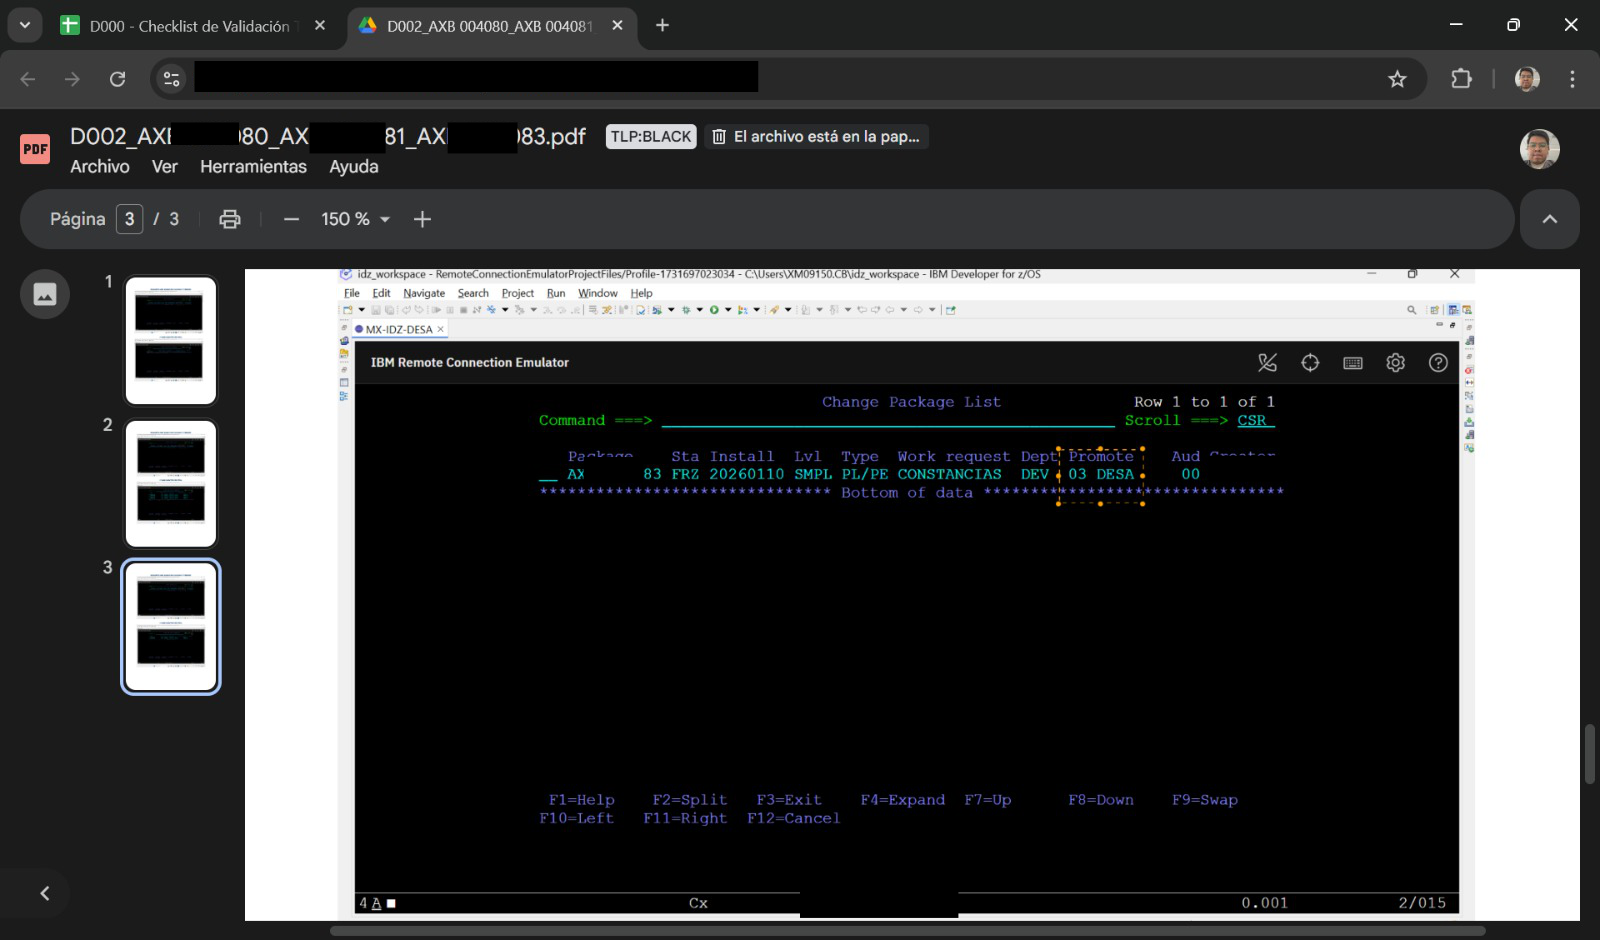
\includegraphics[width=0.95\textwidth]{E8/A8_3}
    \caption{Evidencia gráfica asociada al proceso de validación técnica, utilizada como soporte documental para la revisión de actividades y resultados.}
\end{figure}

\begin{figure}[H]
    \centering
    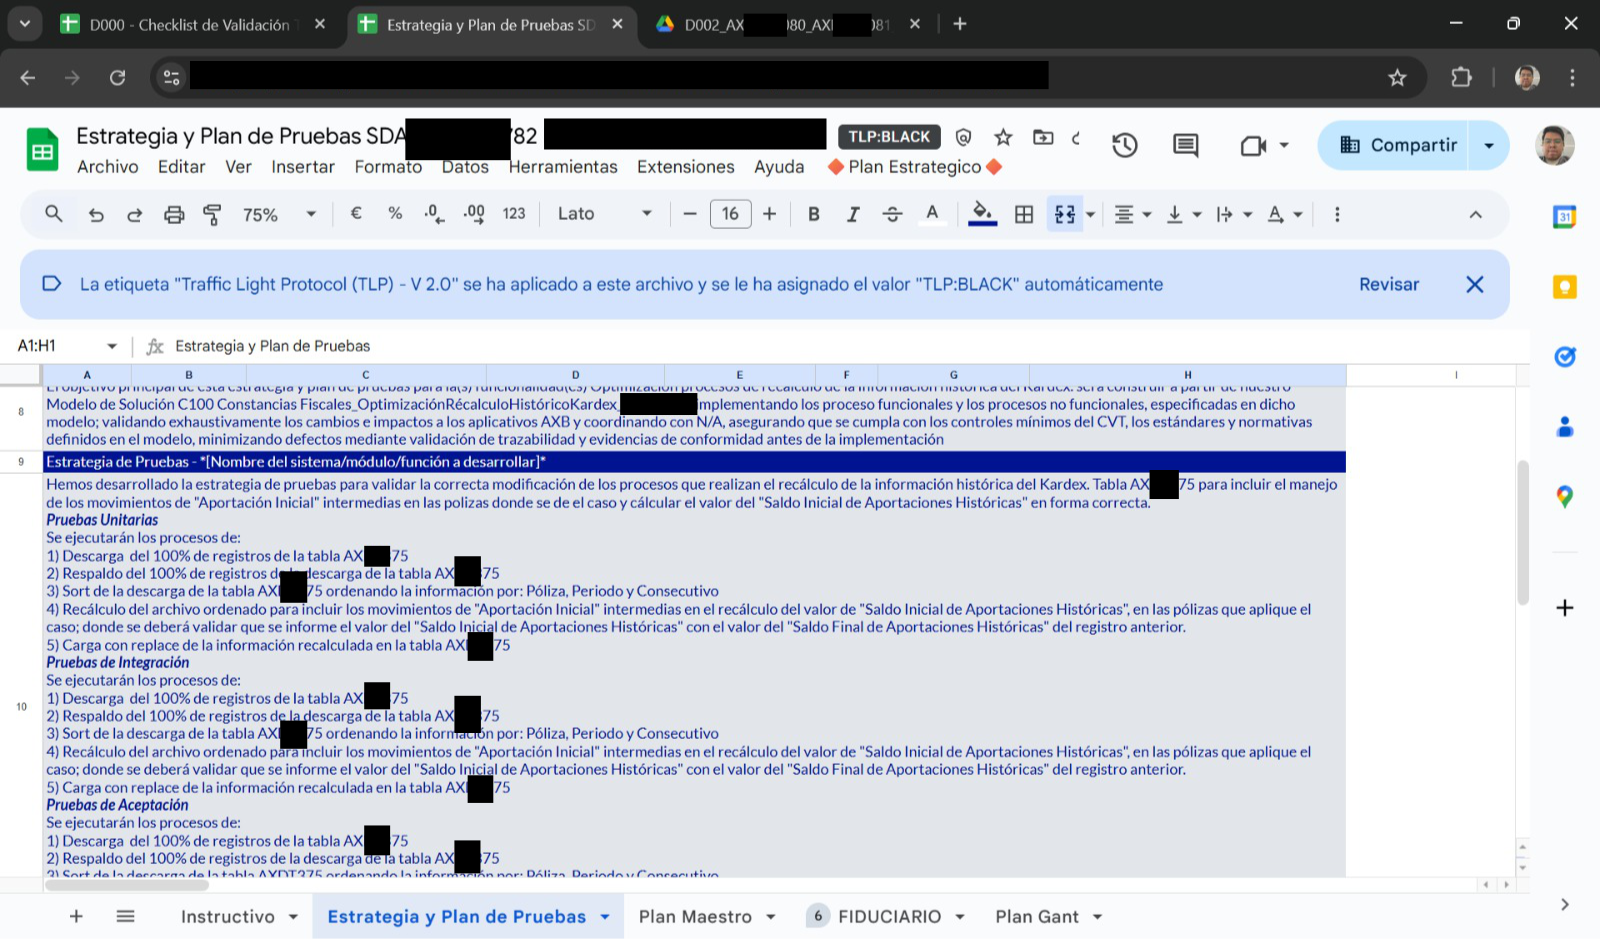
\includegraphics[width=0.95\textwidth]{E8/A8_4}
    \caption{Documento de estrategia y plan de pruebas elaborado en hoja de cálculo, donde se describen los tipos de pruebas, actividades y criterios de validación.}
\end{figure}

\begin{figure}[H]
    \centering
    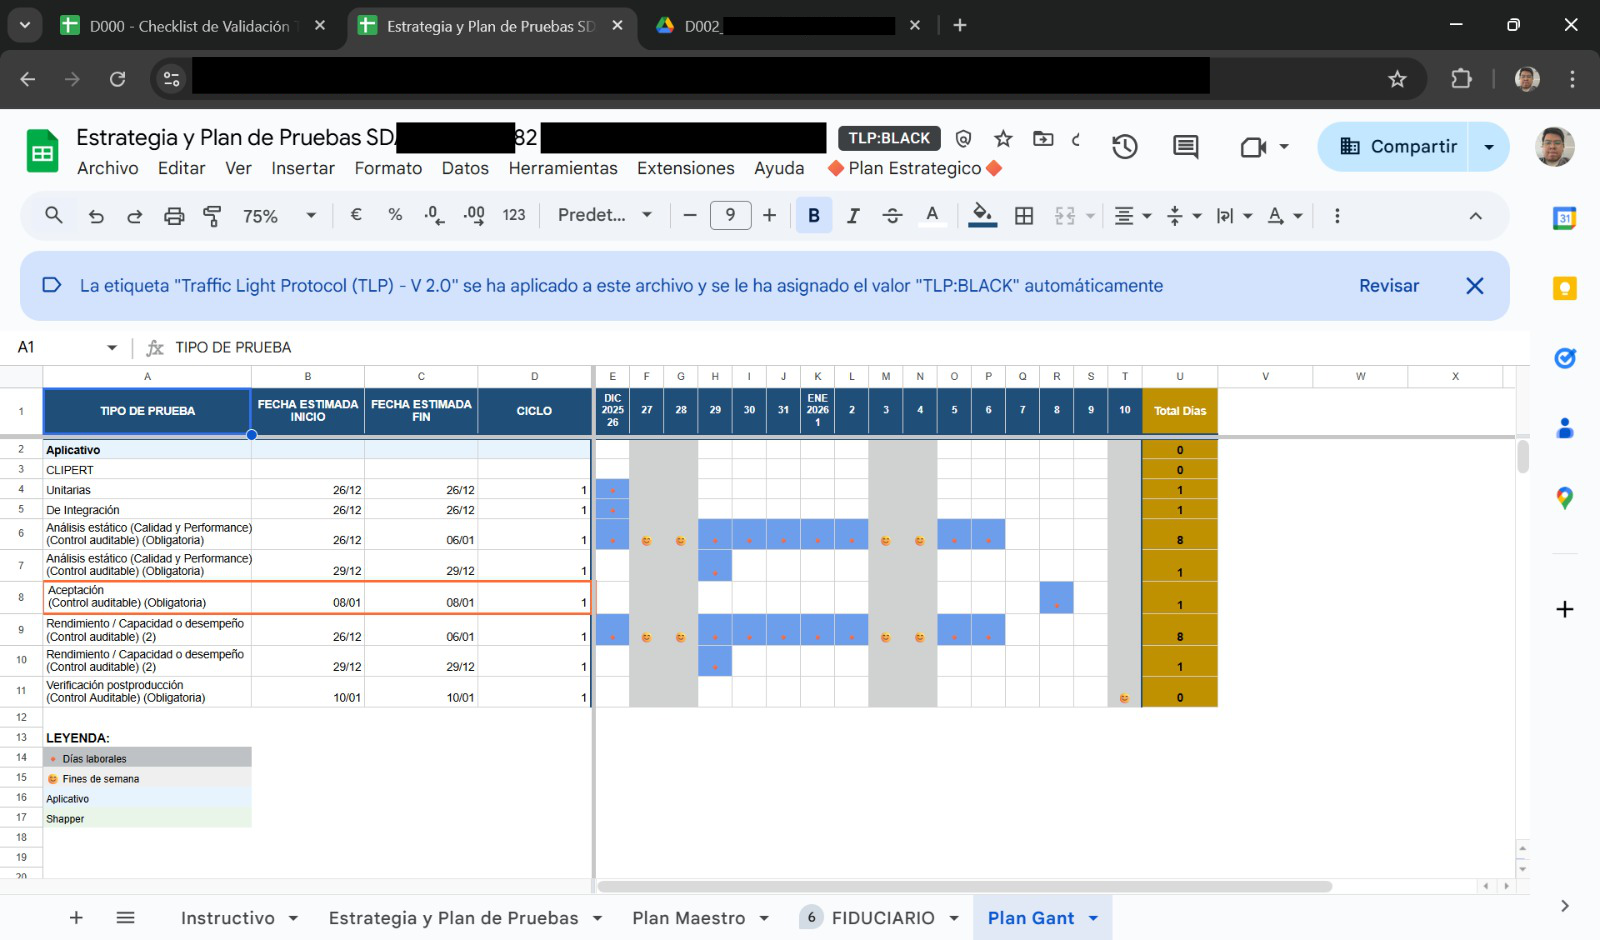
\includegraphics[width=0.95\textwidth]{E8/A8_5}
    \caption{Planeación temporal de actividades de prueba representada mediante un esquema tipo Gantt, utilizada para el seguimiento del avance y tiempos estimados.}
\end{figure}

\begin{figure}[H]
    \centering
    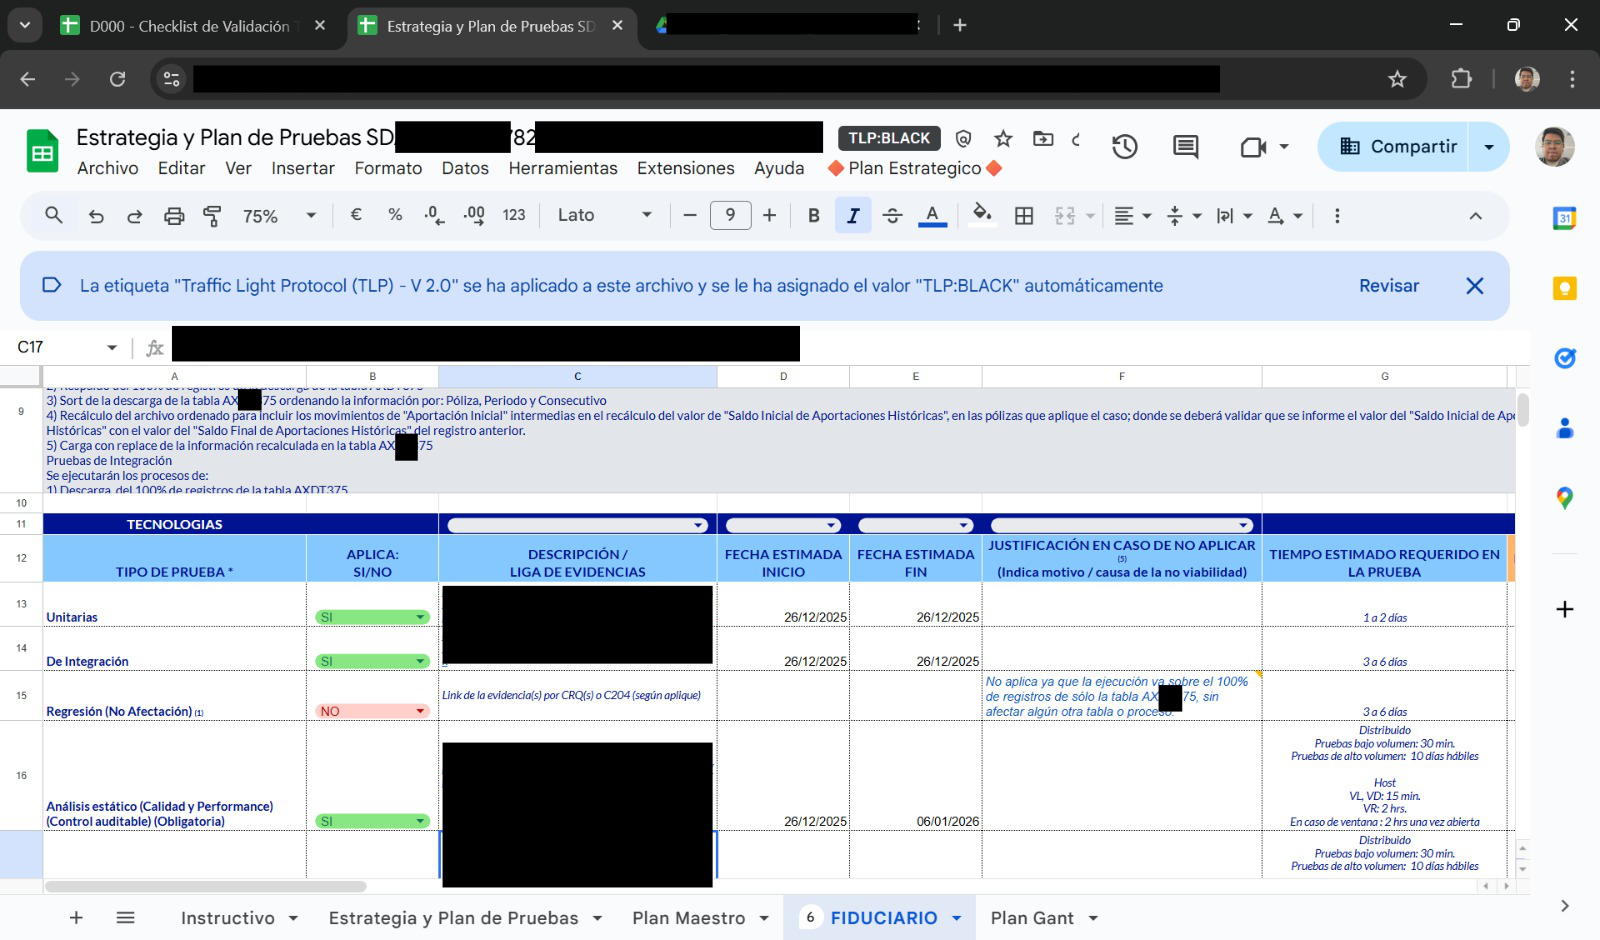
\includegraphics[width=0.95\textwidth]{E8/A8_6}
    \caption{Matriz de tipos de prueba documentada para registrar aplicabilidad, fechas estimadas y justificaciones, como parte del control del proceso de pruebas.}
\end{figure}

\begin{figure}[H]
    \centering
    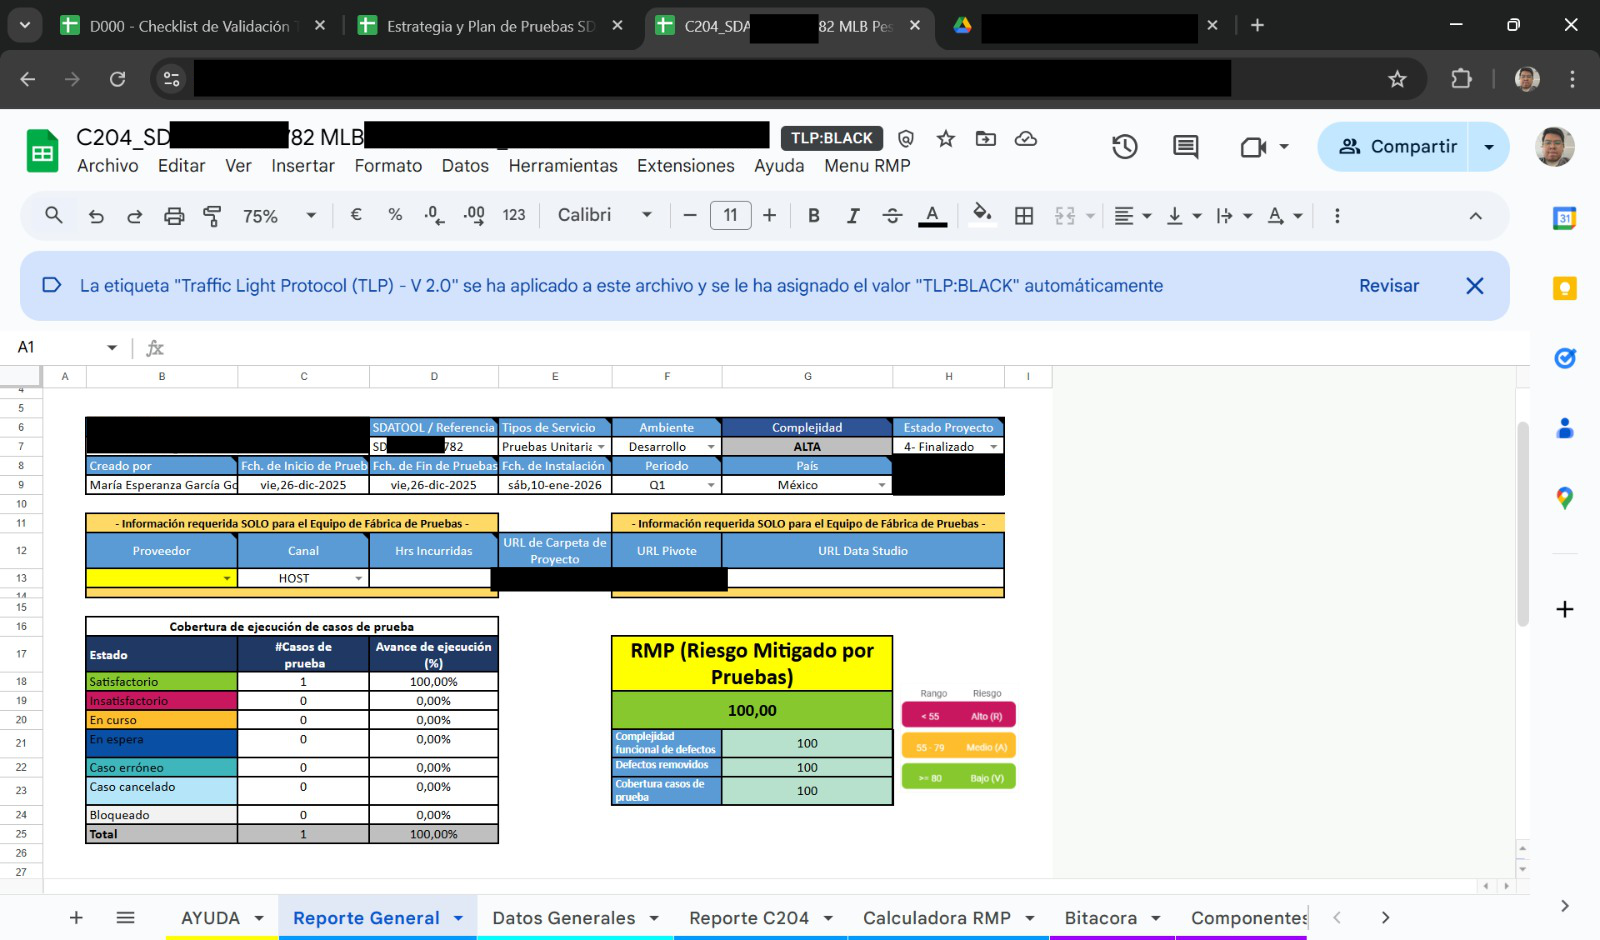
\includegraphics[width=0.95\textwidth]{E8/A8_7}
    \caption{Reporte general de ejecución de pruebas, utilizado para consolidar resultados, avances y métricas asociadas al proceso de validación.}
\end{figure}

\begin{figure}[H]
    \centering
    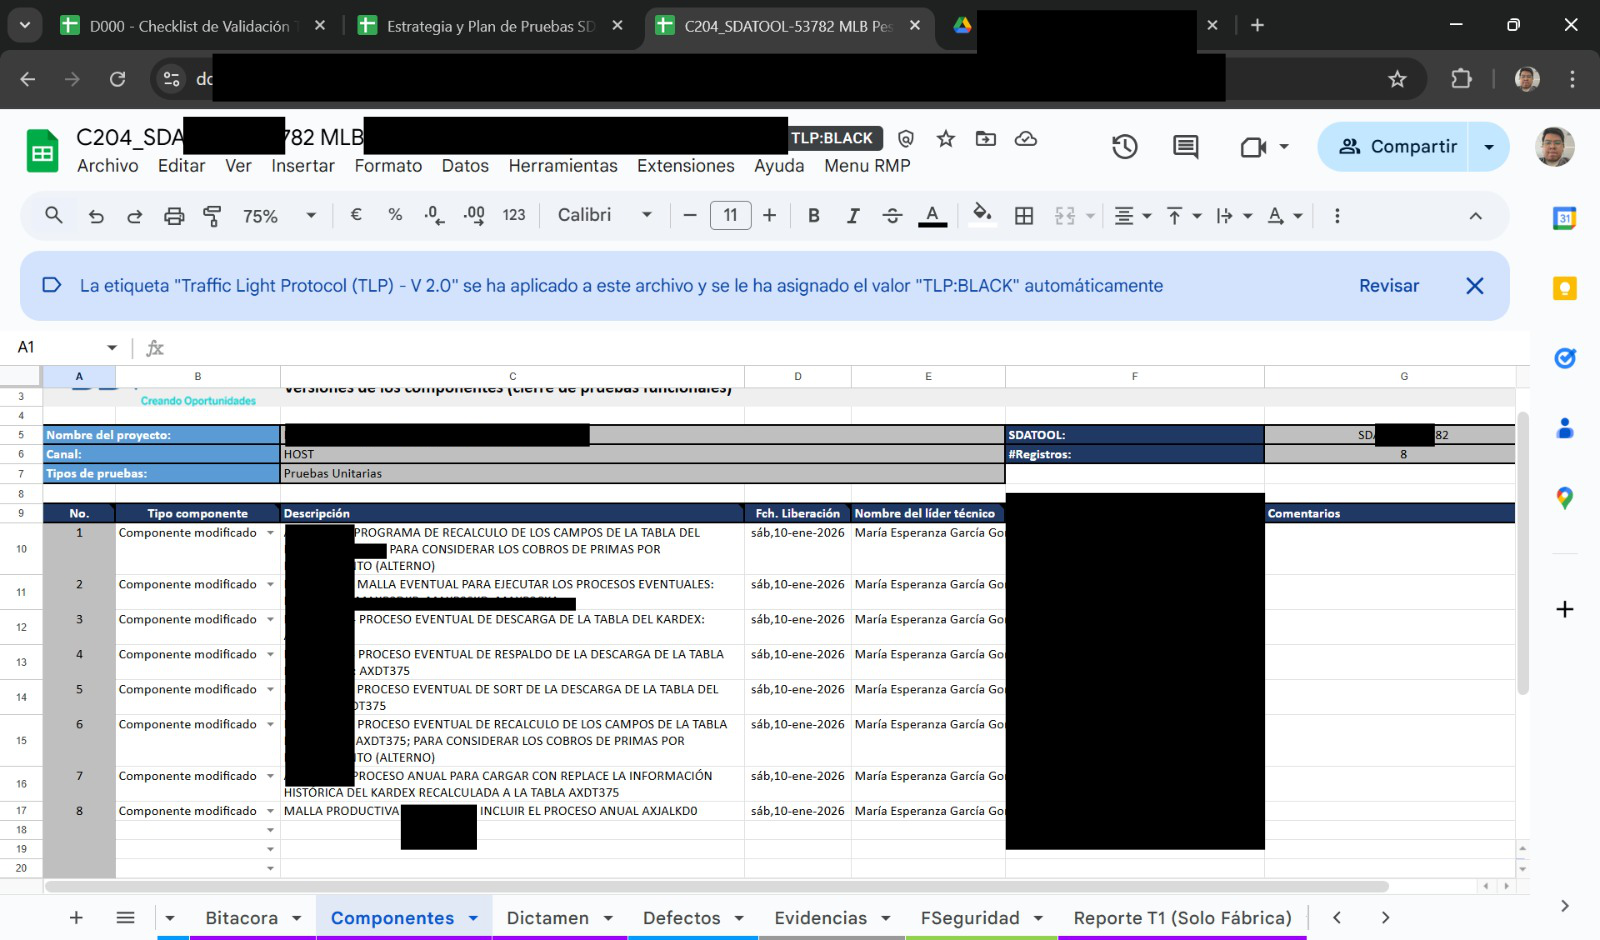
\includegraphics[width=0.95\textwidth]{E8/A8_8}
    \caption{Registro de componentes documentados en hoja de cálculo, donde se describen elementos técnicos, fechas y responsables de validación.}
\end{figure}

\begin{figure}[H]
    \centering
    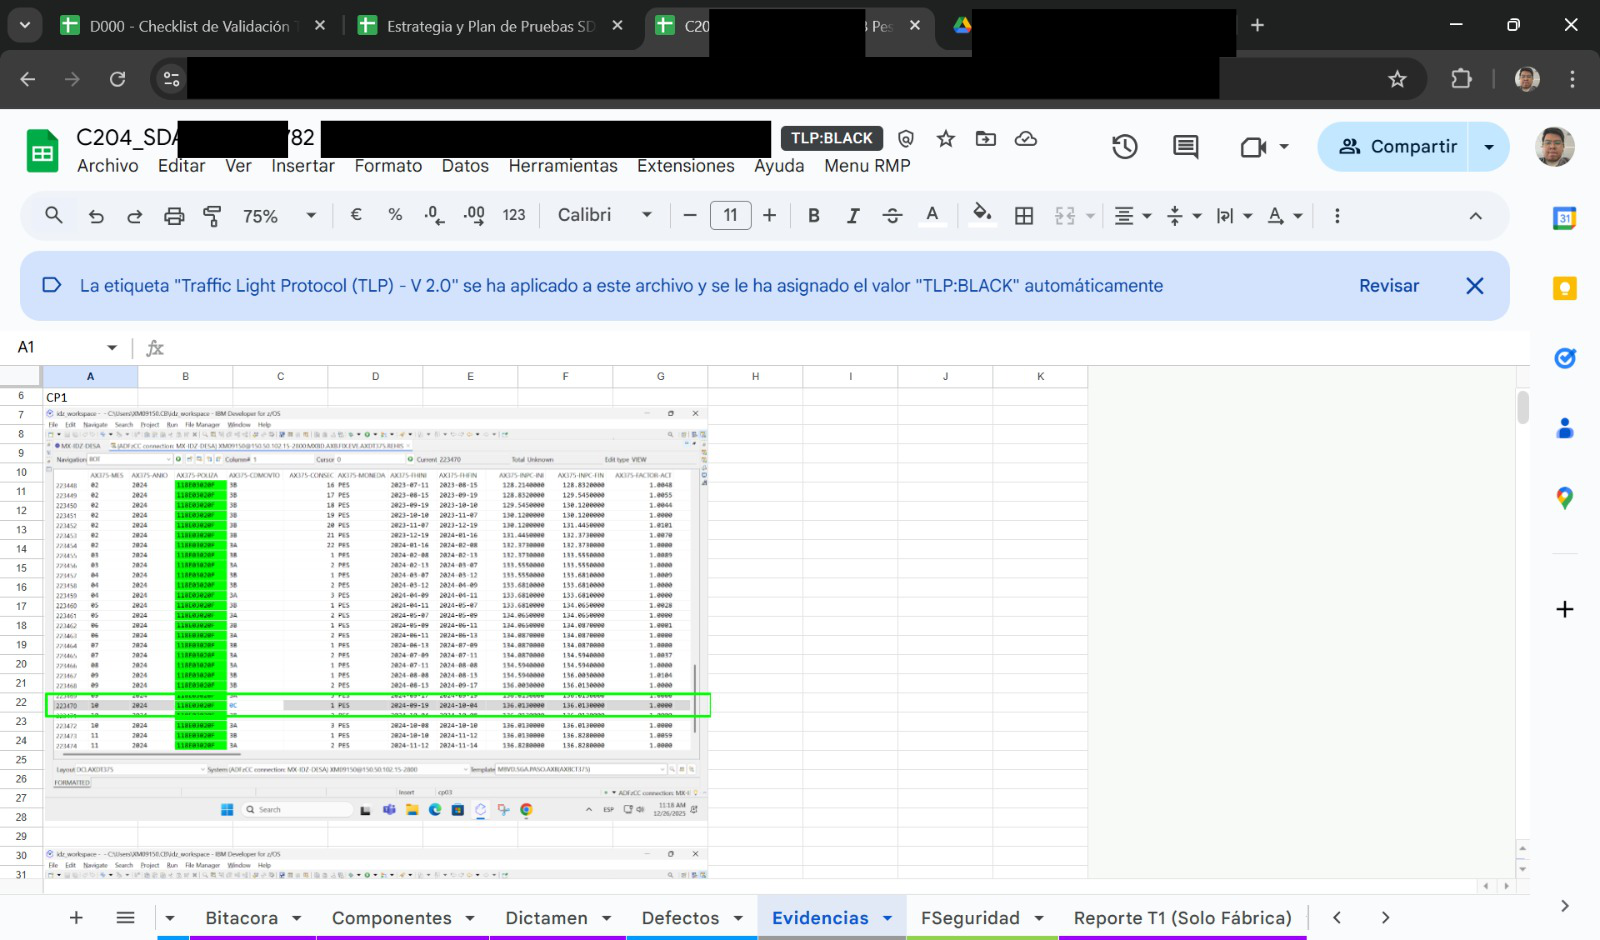
\includegraphics[width=0.95\textwidth]{E8/A8_9}
    \caption{Evidencia gráfica utilizada para respaldar la ejecución de actividades documentadas dentro del proceso de pruebas.}
\end{figure}

\begin{figure}[H]
    \centering
    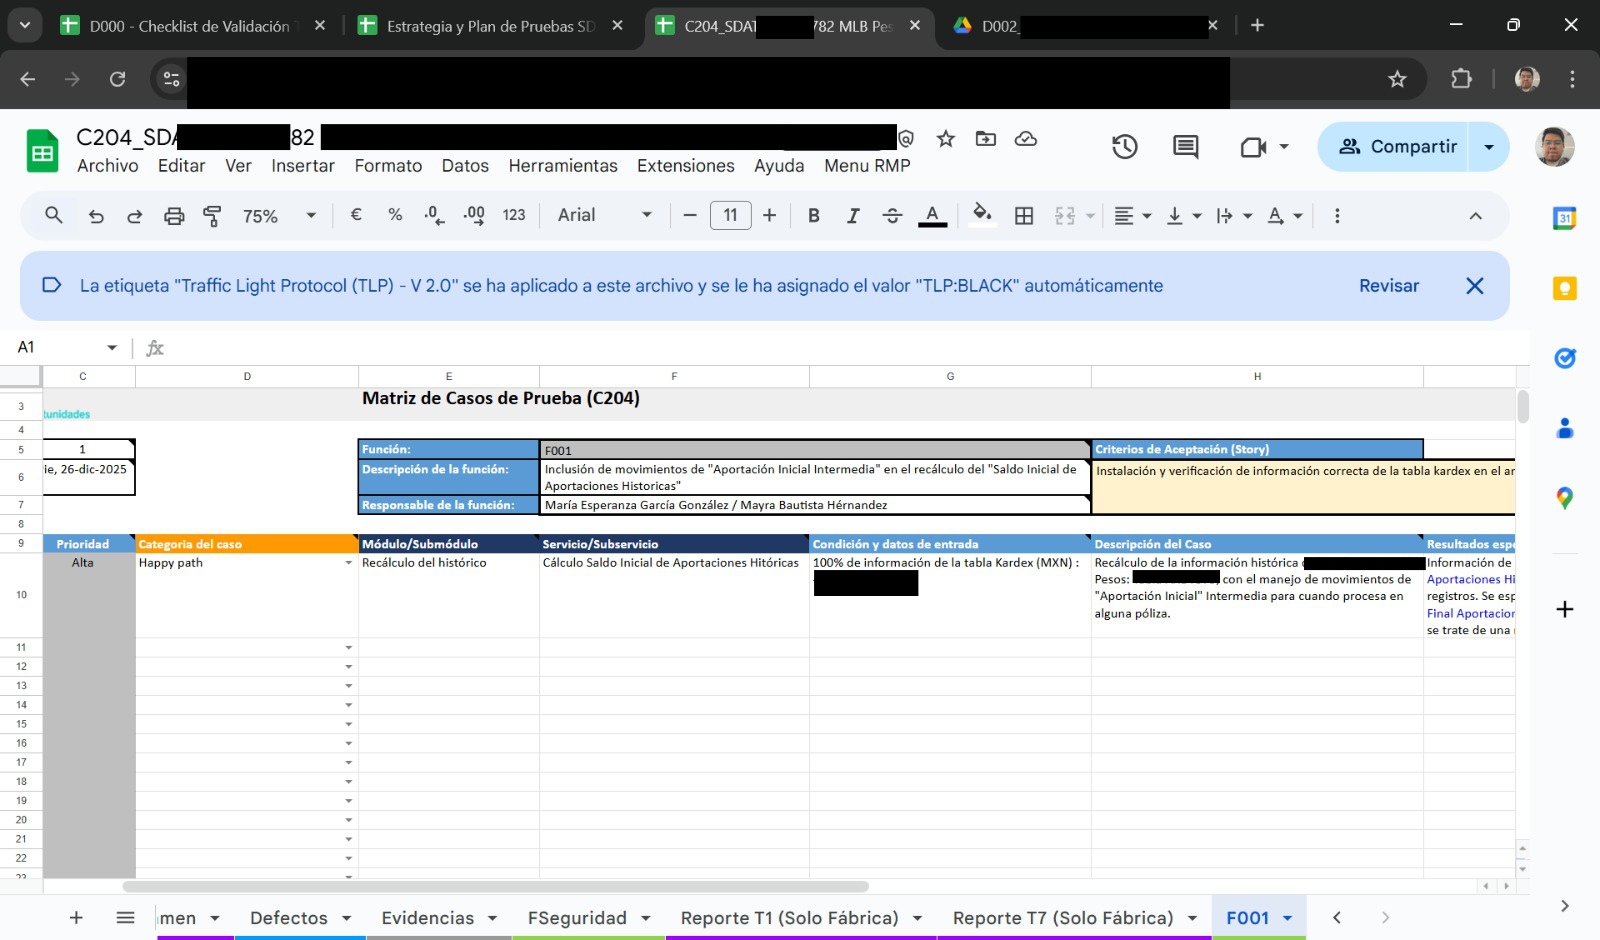
\includegraphics[width=0.95\textwidth]{E8/A8_10}
    \caption{Matriz de casos de prueba documentada, empleada para registrar condiciones de entrada, criterios de aceptación y resultados esperados.}
\end{figure}

\end{document}

